\Chapter{PROSPECT Experiment}
    
    The RAA described in Chapter~\ref{Ch2} leads to the need of an experiment able to probe the short baseline sterile neutrino oscillation, as well as direct measurement of the flux and spectrum of a single fission fuel reactor. 
    The experiment has to meet the requirements of 
    \begin{itemize}
        \item Sub-10~m baseline from a reactor with compact reactor size. 
        \item Fission reactor whose neutrino production is from a single isotope.
        \item High IBD position reconstruction for oscillation measurement.
        \item High energy resolution to precisely measure neutrino spectrum.
    \end{itemize}
    
    PROSPECT~\cite{bib:prospect_physics, bib:prospect_nim}, the Precision Reactor Oscillation and SPECTrum experiment, was designed and built to direct measure neutrino fluxa and spectrum from the High Flux Isotope Reactor (HFIR) located at Oak Ridge National Laboratory (ORNL), USA. 
    PROSPECT's antineutrino detector (AD) covers various baseline from 7~m to 9~m with segmented LS.
    The goal of PROSPECT is to probe the $\sim$1~eV scale sterile neutrino oscillation by the observation of \nuebar disappearance, and precisely measure reactor neutrino spectrum from only $^{235}$U.
    
\Section{HFIR Reactor}

    HFIR reactor is a high enrichment $^{235}$U (HEU) research fission reactor, whose $^{235}$U enrichment is 93\% in average.
    The key parameters of HFIR reactor for PROSPECT neutrino measurement are shown in Table~\ref{tab:HFIR}.
\begin{table}[h]
    \centering
    \caption[HFIR parameters]{The properties of the HFIR reactor.}
    \begin{tabular}{cc}
    \hline
    \hline
    Parameter  & Value   \\
    \hline
    Power    & 85~MW \\
    Dimensions     & 435~mm (diameter) $\times$ 508~mm (height) \\
    $^{235}$U enrichment & 93\% \\
    Neutrino source & $\sim$99\% from $^{235}$U \\
    Reactor cycle & $\sim$25~day on, $\sim$30~day off \\
    \hline
    \end{tabular}

\label{tab:HIFR}
\end{table}

\begin{figure}
    \centering
    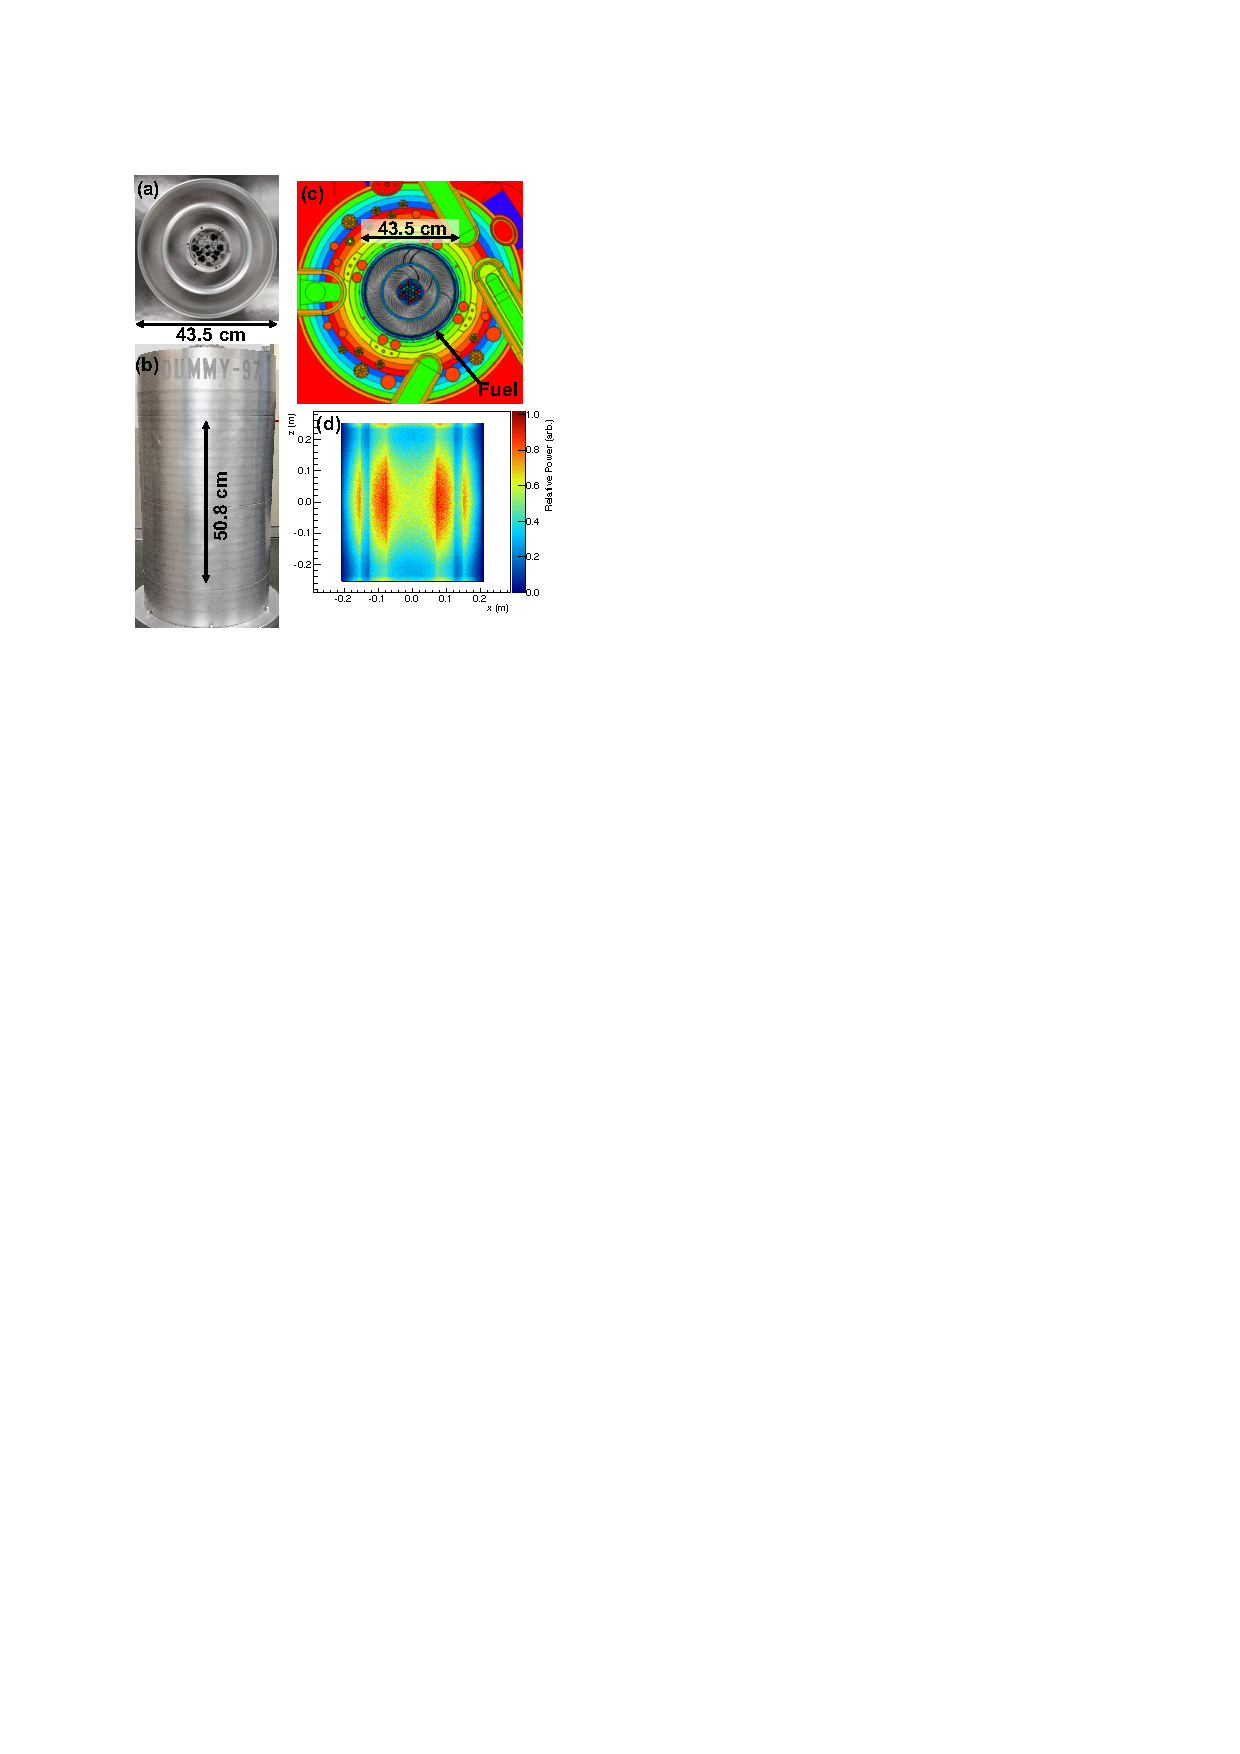
\includegraphics[width=0.5\textwidth]{Figures/HFIR.pdf}
    \caption[The dimensions and power distribution of HFIR]{A model of the reactor~\cite{bib:prospect_nim} parameters (a) and (b) are the diameter and height of the HFIR core.
    The location of the HFIR core in a detailed reactor system simulation is indicated in (c).
    (d) is a projection of the fission power density of HFIR at the x-z plane.}
    \label{fig:HFIR}
\end{figure}

    HFIR is a cylindrical fission reactor.
    Its compact size, as shown in Table~\ref{tab:HFIR} and Figure~\ref{fig:HFIR}, is ideal to limit the uncertainty of baseline.
    To maintain its high $^{235}$U enrichment, the HFIR reactor has relatively short reactor cycles.
    In this case, the fuel evolution of fissile isotopes is negligible.
    
    The HFIR facility also brought unique challenge of background for neutrino measurement. 
    Because of the very short baseline requirement of the experiment and availability of the experiment site, the PROSPECT AD is exposed to cosmic ray background with minimal overburden. 
    The detector also faces reactor correlated background, e.g. the neutron background generated from reactor and the $\gamma$ ray background from the metallic materials in the piping of the facility.
    A comprehensive background characterization is therefore organized in the research and development (R\&D) phase of PROSPECT~\cite{bib:prospect_background}. 
    The detector and additional background shielding was designed based on the by this background survey.
    
\begin{figure}
    \centering
    %\vspace{0pt}
    \includegraphics[width=0.47\textwidth, valign=t]{Figures/NeutronBGMap.pdf}
    %\vspace{0pt} 
    \includegraphics[width=0.51\textwidth, valign=t]{Figures/GammaBGMap.pdf}
    \caption[Local background distribution at HFIR facility]{(Left) The reactor correlated neutron background rate (nSv/h) shown in a map of the HFIR site where PROSPECT is deployed.
    (Right) The local $\gamma$ ray background rate (Hz) shwon in the same map.
    }
    \label{fig:prospect_background}
\end{figure}

\Section{Detector Design}

    The PROSPECT AD is a $\sim$4~ton $^{6}$Li-doped LS ($^{6}$LiLS) detector deployed at 7-9~m baselines from the HFIR core.
    The key parameters of the PROSPECT AD is shown in Table~\ref{tab:PROSPECT_AD}.
    The schematic of detector deployment at the HFIR facility is shown in Figure~\ref{fig:PROSPECT_LAYOUT}.
\begin{table}[h]
    \centering
    \caption[PROSPECT AD Parameters]{The key parameters of the PROSPECT AD~\cite{bib:prospect_nim}.}
    \begin{tabular}{cc}
    \hline
    \hline
    Parameter  & Value   \\ 
    \hline
    Target volume \& mass    & 3760 litters, 3.68 tons\\
    Target dimension & 1.176\,m wide $\times$ 2.045\,m long  $\times$ 1.607\,m tall \\
    Baseline     & 7.9~m \\
    Liquid scintillator & EJ-309 based LS with $<$0.1\% $^{6}$Li \\
    LS energy resolution & 4.5\% \\
    Segments & 14 horizontal $times$ 11 vertical \\
    Segment dimension & 1.176\,m wide $\times$ 14.5~cm long  $\times$ 14.5~cm tall \\
    Light collection & diameter = 12.7~cm (5~inch) PMTs\\
    \hline
    \end{tabular}
    \label{tab:PROSPECT_AD}
\end{table}
\begin{figure}
    \centering
    %\vspace{0pt}
    \includegraphics[width=0.6\textwidth]{Figures/Layout.pdf}
    \caption[The layout of the PROSPECT experiment]{The layout of the PROSPECT experiment.
    The PROSPECT AD is deployed 7.9~m from the reactor center to the detector center.
    Additional on site shield was installed between the reactor pool and the AD to eliminate the local $\gamma$ ray background.
    }
    \label{fig:PROSPECT_LAYOUT}
\end{figure}
    
    The anatomy of the PROSPECT AD is shown in Figure~\ref{fig:PROSPECT_AD}.
    The inner volume of detector is contained in a liquid tight acrylic vessel filled with the $^{6}$LiLS, which is made from an EJ-309 base, an organic LS \cite{bib:lspaper}.
    The designed energy resolution is 4.5\% to optimize PROSPECT's IBD spectrum measurement.
    An advantage of utilizing the EJ-309 is the pulse shape discrimination (PSD) feature making the PROSPECT AD sensitive to particle identity, which is described in detail in Section~\ref{sec:detection}.
    The $^{6}$Li is loaded as a main neutron capture isotope.

\begin{figure}
    \centering
    %\vspace{0pt}
    \includegraphics[trim = 0cm 2cm 0cm 2cm, clip,width=0.6\textwidth]{Figures/DetectorDesign.pdf}
    \caption[The design of PROSPECT AD]{The design of PROSPECT AD consisting the inner detector and the shielding.
    The inner detector includes $^{6}$LiLS, the optical grid, photomultiplier tubes (PMTs), and the calibration system.
    }
    \label{fig:PROSPECT_AD}
\end{figure}

    The inner volume of the PROSPECT AD is optically segmented by a light weight optical grid subsystem~\cite{bib:prospect_og}.
    The optical grid consist of highly reflective carbon fiber backed separators dividing the LS volume into 14$\times$11 identical longitudinal segments. 
    The ends of each segments are enclosed by two diameter = 12.7~cm photomultiplier tubes (PMTs).
    The 
    The segment with largest LS light yield is identified as the interaction point (x- and y-direction) of an incident particle.
    The readout of PMT housed in mineral-oil filled acrylic modules (PMT optical modules) on both sides of each segment, allowing for timing- and charge-based position reconstruction along the axis (z-direction) of each segment~\cite{bib:prospect_50, bib:P20}.
    Hence, the optical grid made PROSPECT AD able to reconstruct incident particles' track and 3D position, which is an essential function for the cosmic ray rejection and the oscillation measurement in the baseline between 7~m to 9~m.
    
\Section{Antineutrino Detection}
\label{sec:detection}

\Section{Optical Grid}
\label{sec:OG}

\Section{Background Shielding}

\Section{Calibration System}

\Section{Detector Construction and Commissioning}

\Section{Data Acquisition}